\section{Change in the Christensen-Burley profile to better fit Monte
Carlo references}

\textit{Note about Monte Carlo references:
There are consistent results achieved for Searchlight experiment
(semi-infinite slab with narrow pencil beam of light pointing from top in the normal
direction). In which brute force Monte-Carlo simulation in P2 (path tracing) was
compared to PTDL approach and also to hybrid technique used in Mitsuba
renderer. All three methods produce the same result in the scope of their
capabilities. It give us some assurance of the correctness of the Monte-Carlo
algorithms which are used as the references.}


\begin{figure}
    \centering
    \begin{subfigure}{0.48\textwidth}
        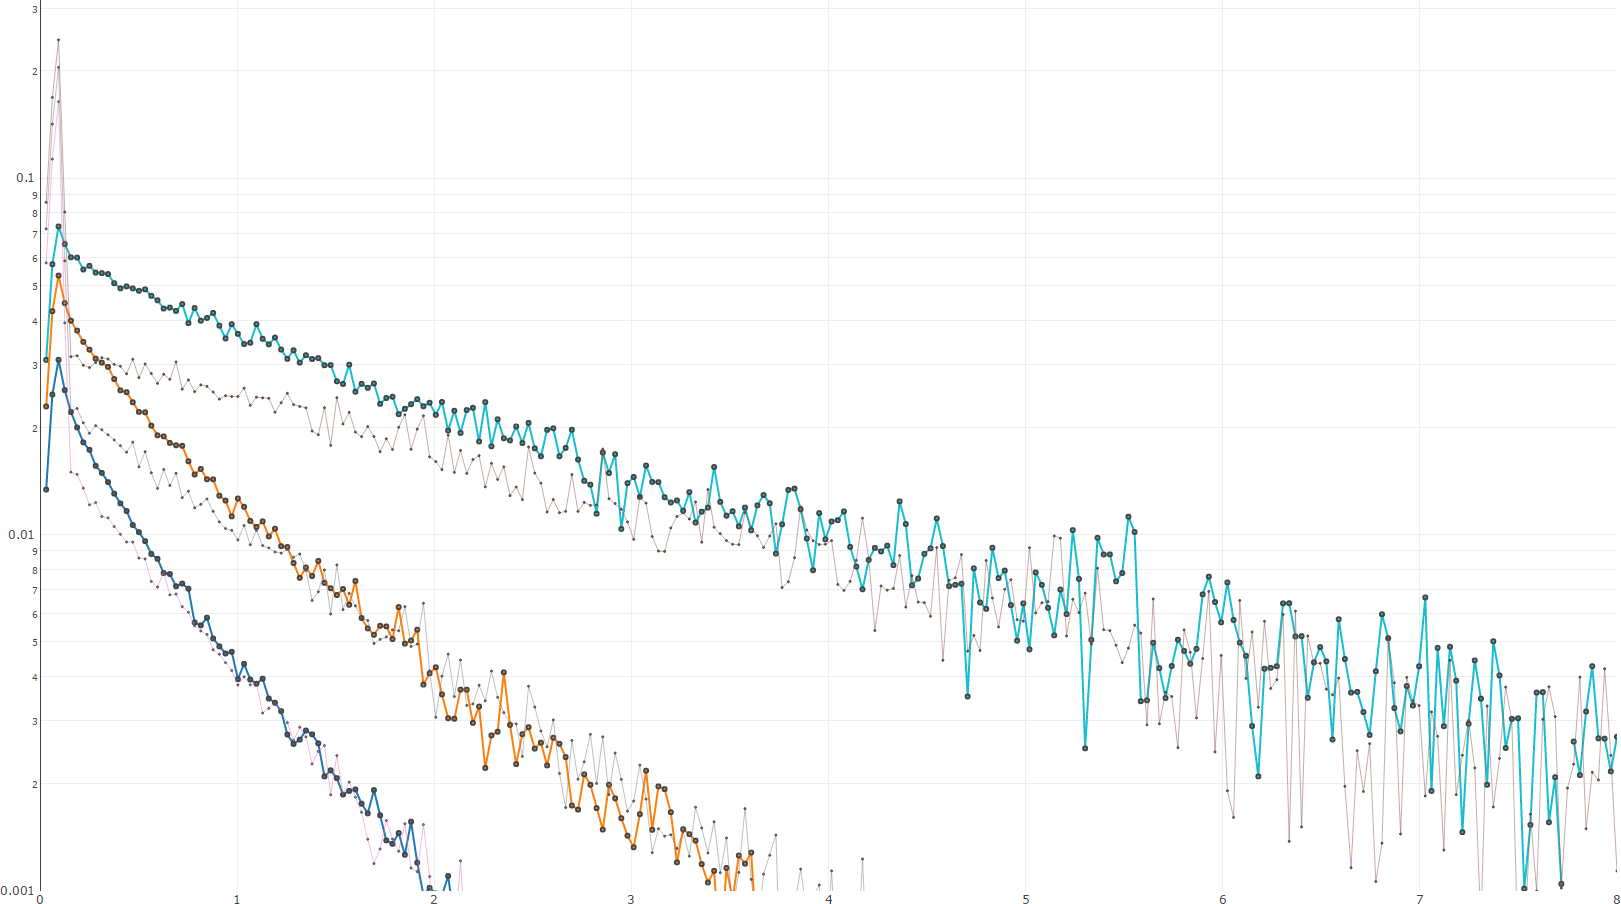
\includegraphics[width=\textwidth]{imgs/plots/burley_old_fitting}
        \caption{Original Christensen-Burley}
    \end{subfigure}
    \quad
    \begin{subfigure}{0.48\textwidth}
        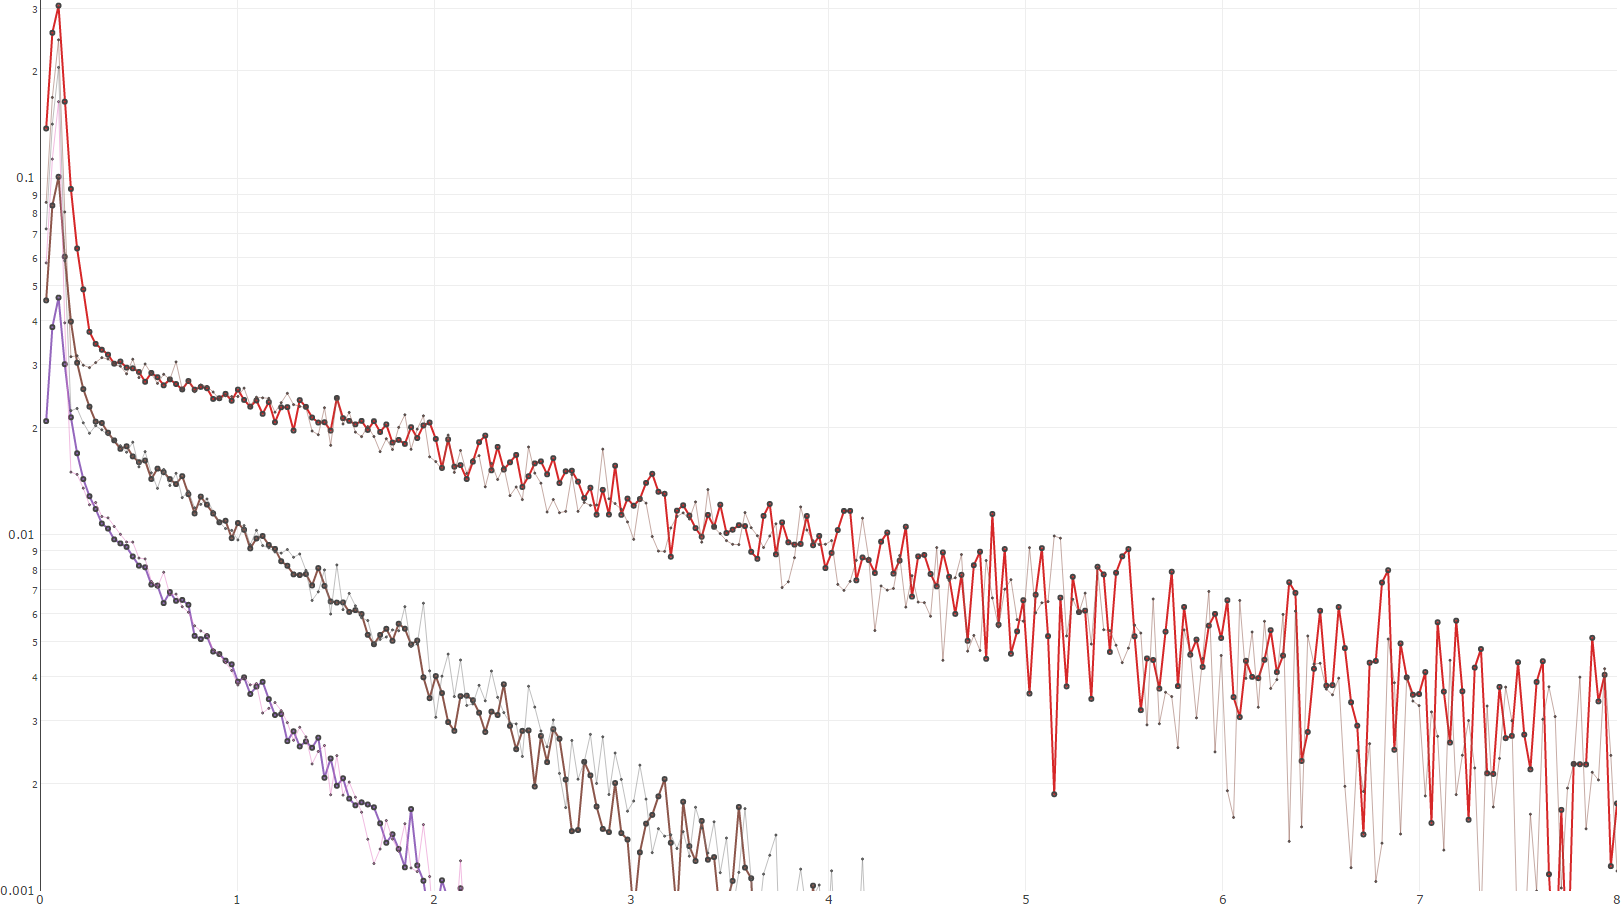
\includegraphics[width=\textwidth]{imgs/plots/burley_new_fitting}
        \caption{Proposed}
    \end{subfigure}

    \caption{Comarison between the original and proposed techniques in log-y
    scale. Monte Carlo references are inthin lines. TODO: make clear plots and
    accompany them with rendered images}
    \label{fig:burley_fitting}
\end{figure}

As we can see from the graph \ref{fig:burley_fitting}, there is a tendency for
the original model to overestimate outgoing radiant exitance in the region close
to the light source (around $x\leq=3$). This trend was observed in many
experiments with different optical properties of the material.

The proposed model has different the factorization of the exponents than the
original \gls{BSSRDF} profile. Instead of using unified parameter $s$, I propose
to split it into two factors for each of the exponent:

\begin{equation}\label{eq:burley_modified}
R_{l=1}(r) = A\dfrac{se^{-sr}+te^{-tr/3}}{8\pi r}
\end{equation}

It still allows to easily normalize the model and use the same technique for
importance sampling. The particular form of s and t is based on the original
function developed by Christensen et al., but has a linear function coefficient
to get better results.

\ldots